\documentclass[12pt,letterpaper,oneside]{report}

\usepackage[spanish]{babel}
\usepackage{fontspec}

\setmainfont{Times New Roman}
\setmonofont{Menlo}

\usepackage[letterpaper,margin=1in]{geometry}
\usepackage{setspace}

\onehalfspacing

\usepackage{graphicx}
\usepackage{float}
\usepackage{caption}
\usepackage{listings}
\usepackage{hyperref}
\usepackage{titlesec}

\titleformat{\chapter}[display]{\normalfont\bfseries\fontsize{24}{28}\selectfont}{}{0pt}{}
\hypersetup{colorlinks=true,linkcolor=black,urlcolor=black}
\captionsetup{font=small,justification=centering}

\setlength{\parindent}{0pt}
\setlength{\parskip}{6pt}
\renewcommand{\lstlistingname}{Código}

\lstset{
  basicstyle=\ttfamily\fontsize{9}{10}\selectfont,
  frame=single,
  numbers=left,
  numberstyle=\tiny,
  breaklines=true,
  columns=fullflexible,
  captionpos=b,
  showstringspaces=false
}

\titlespacing*{\chapter}{0pt}{0pt}{5pt}
\titlespacing*{\section}{0pt}{3pt}{3pt}

\begin{document}

\begin{titlepage}
\centering

\includegraphics[height=2.5in]{figuras/UAT-Escudo.jpeg}\par
\vspace{1.5cm}
{\bfseries\fontsize{16}{18}\selectfont Tarea 1\par}
\vspace{-0.2cm}
{\bfseries\fontsize{16}{18}\selectfont Codificación de programas básicos\par}
\vspace{1cm}
{\bfseries\fontsize{16}{18}\selectfont Análisis y Diseño de Algoritmos\par}
\vspace{-0.2cm}
{\bfseries\fontsize{16}{18}\selectfont Maestría en Ciencias e Ingeniería de Datos\par}
\vspace{1cm}
{\fontsize{14}{16}\selectfont Alumno: Rodrigo Piña Enríquez\par}
\vspace{-0.2cm}
{\fontsize{14}{16}\selectfont Profesor: Dr. José Lázaro Martínez Rodríguez\par}
\vfill

\includegraphics[height=0.7in]{figuras/FIC-03.png}\par
\vspace{0.5cm}
{\fontsize{14}{16}\selectfont Septiembre 2026\par}
\end{titlepage}

\tableofcontents
\clearpage

% ============================== PROBLEMA 1 ==============================

\chapter*{1. Invertir y transponer una matriz}
\addcontentsline{toc}{chapter}{1. Invertir y transponer una matriz}

\setcounter{chapter}{1}
\setcounter{section}{0}

\section{Problema}

Invertir una matriz y hallar la transpuesta de una matriz.

\section{Solución}

Se implementaron dos funciones en Rust. La función \texttt{flip} intercambia los
elementos simétricos de la matriz para invertir su orden. La función
\texttt{transpose} intercambia filas por columnas y genera una nueva matriz
transpuesta.
\vspace{10pt}

\lstinputlisting[
  firstline=1,
  lastline=32,
  caption={Funciones para invertir y transponer una matriz},
  label={cod:matriz}
]{../algoritmos/src/matrix.rs}

\clearpage

\section{Pruebas de ejecución}
Para ambas pruebas se utilizó la matriz de $2 \times 3$ con los valores
\texttt{[1, 2, 3]} y \texttt{[4, 5, 6]}.

\begin{figure}[H]
\centering
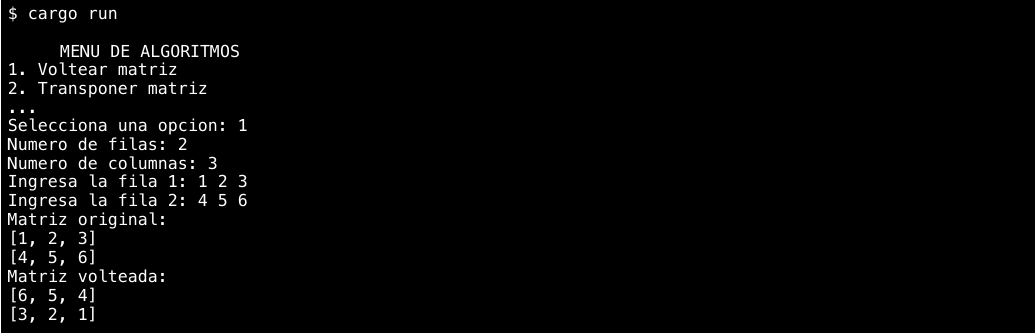
\includegraphics[width=\textwidth]{figuras/pruebas/inversion_matriz.png}
\caption{Ejecución de la opción para invertir la matriz.}
\label{fig:inversion-matriz}
\end{figure}

\begin{figure}[H]
\centering
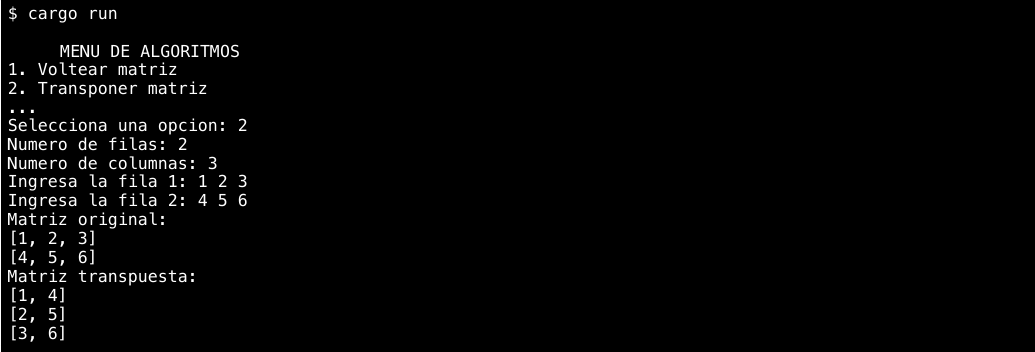
\includegraphics[width=\textwidth]{figuras/pruebas/transpuesta_matriz.png}
\caption{Ejecución de la opción para obtener la matriz transpuesta.}
\label{fig:transpuesta-matriz}
\end{figure}

% ============================== PROBLEMA 2 ==============================

\clearpage
\chapter*{2. Ordenamiento burbuja}
\addcontentsline{toc}{chapter}{2. Ordenamiento burbuja}
\setcounter{chapter}{2}
\setcounter{section}{0}

\section{Problema}

Ordenación de la burbuja.

\section{Solución}

Se implementó el método de burbuja para ordenar un vector de números enteros
de menor a mayor.
\vspace{10pt}

\lstinputlisting[
  caption={Función de ordenamiento burbuja},
  label={cod:burbuja}
]{../algoritmos/src/bubble.rs}

\section{Pruebas de ejecución}

Se ordenó el vector \texttt{[5, 3, 8, 1, 2]}.

\begin{figure}[H]
\centering
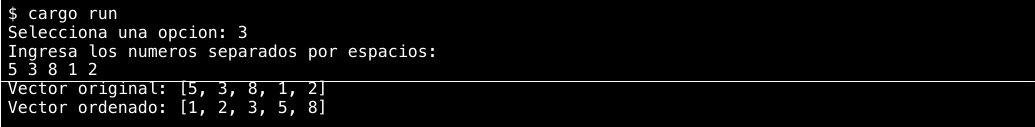
\includegraphics[width=\textwidth]{figuras/pruebas/burbuja.png}
\caption{Ejecución del ordenamiento burbuja.}
\label{fig:burbuja}
\end{figure}

% ============================== PROBLEMA 3 ==============================
\clearpage
\chapter*{3. Convertir números romanos a enteros}
\addcontentsline{toc}{chapter}{3. Convertir números romanos a enteros}
\setcounter{chapter}{3}
\setcounter{section}{0}

\section{Problema}

Convertir romanos en números enteros.

\section{Solución}

Se implementó una función que obtiene el valor de cada símbolo romano y los
suma o resta de acuerdo con el símbolo siguiente.
\vspace{10pt}

\lstinputlisting[
  caption={Funciones para convertir un número romano a entero},
  label={cod:romano}
]{../algoritmos/src/roman_to_number.rs}

\section{Pruebas de ejecución}

Se utilizó el número romano \texttt{MCMXCIV}, cuyo equivalente es 1994.

\begin{figure}[H]
\centering
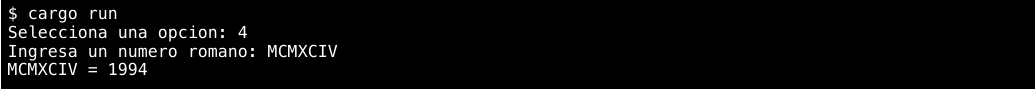
\includegraphics[width=\textwidth]{figuras/pruebas/romano.png}
\caption{Ejecución de la conversión de número romano a entero.}
\label{fig:romano}
\end{figure}

% ============================== PROBLEMA 4 ==============================
\clearpage
\chapter*{4. Máximo común divisor}
\addcontentsline{toc}{chapter}{4. Máximo común divisor}
\setcounter{chapter}{4}
\setcounter{section}{0}

\section{Problema}

Hallar el MCD (máximo común divisor) de dos números.

\section{Solución}

Se implementó el algoritmo de Euclides para calcular el máximo común divisor
de dos números enteros.
\vspace{10pt}

\lstinputlisting[
  caption={Función para calcular el máximo común divisor},
  label={cod:mcd}
]{../algoritmos/src/mcd.rs}

\section{Pruebas de ejecución}

Se calcularon los divisores comunes de 48 y 18.

\begin{figure}[H]
\centering
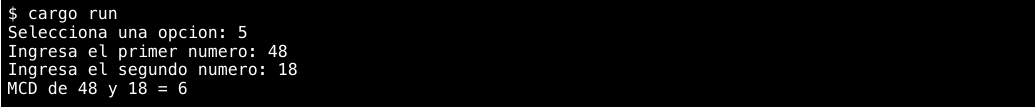
\includegraphics[width=\textwidth]{figuras/pruebas/mcd.png}
\caption{Ejecución del cálculo del máximo común divisor.}
\label{fig:mcd}
\end{figure}

% ============================== PROBLEMA 5 ==============================
\clearpage
\chapter*{5. Comprobación de número primo}
\addcontentsline{toc}{chapter}{5. Comprobación de número primo}
\setcounter{chapter}{5}
\setcounter{section}{0}

\section{Problema}

Dado un número $n$, comprobar si es primo o no.

\section{Solución}

Se implementó una función que verifica si el número tiene algún divisor entre
2 y su raíz cuadrada.
\vspace{10pt}

\lstinputlisting[
  caption={Función para comprobar si un número es primo},
  label={cod:primo}
]{../algoritmos/src/prime_number.rs}

\section{Pruebas de ejecución}

Se comprobó que el número 29 es primo.

\begin{figure}[H]
\centering
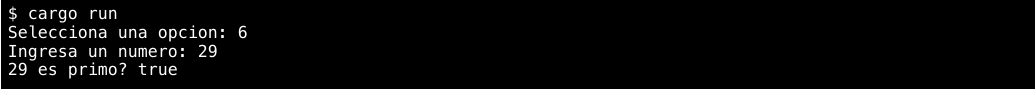
\includegraphics[width=\textwidth]{figuras/pruebas/primo.png}
\caption{Ejecución de la comprobación de número primo.}
\label{fig:primo}
\end{figure}

% ============================== PROBLEMA 6 ==============================
\clearpage
\chapter*{6. Comprobación de palíndromo}
\addcontentsline{toc}{chapter}{6. Comprobación de palíndromo}
\setcounter{chapter}{6}
\setcounter{section}{0}

\section{Problema}

Comprobar si una cadena dada es un palíndromo.

\section{Solución}

Se implementó una función que compara los caracteres de la cadena desde los
extremos hacia el centro.
\vspace{10pt}

\lstinputlisting[
  caption={Función para comprobar si una cadena es palíndromo},
  label={cod:palindromo}
]{../algoritmos/src/palindrome.rs}

\section{Pruebas de ejecución}

Se comprobó que la palabra \texttt{reconocer} es un palíndromo.

\begin{figure}[H]
\centering
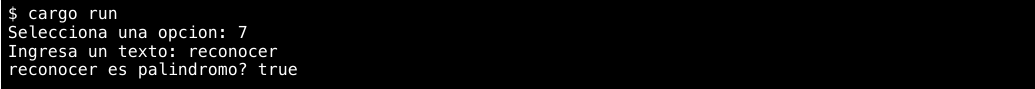
\includegraphics[width=\textwidth]{figuras/pruebas/palindromo.png}
\caption{Ejecución de la comprobación de palíndromo.}
\label{fig:palindromo}
\end{figure}

% ============================== PROBLEMA 7 ==============================
\clearpage
\chapter*{7. Elemento mayor de una matriz}
\addcontentsline{toc}{chapter}{7. Elemento mayor de una matriz}
\setcounter{chapter}{7}
\setcounter{section}{0}

\section{Problema}

Hallar el elemento mayor de una matriz.

\section{Solución}

Se implementó una función que recorre todos los elementos de la matriz y
conserva el valor mayor encontrado.
\vspace{10pt}

\lstinputlisting[
  firstline=33,
  lastline=45,
  caption={Función para obtener el elemento mayor de una matriz},
  label={cod:mayor-matriz}
]{../algoritmos/src/matrix.rs}

\section{Pruebas de ejecución}

Se utilizó una matriz de $2 \times 3$ cuyo elemento mayor es 12.

\begin{figure}[H]
\centering
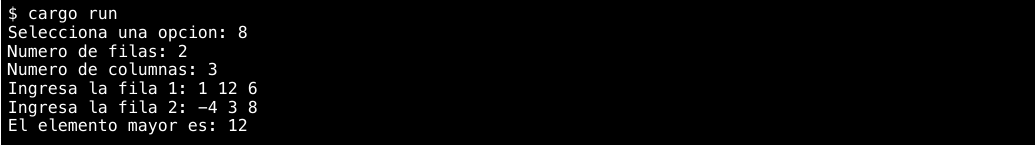
\includegraphics[width=\textwidth]{figuras/pruebas/mayor_matriz.png}
\caption{Ejecución para obtener el elemento mayor de una matriz.}
\label{fig:mayor-matriz}
\end{figure}

\clearpage
\section*{Repositorio del proyecto}
\addcontentsline{toc}{section}{Repositorio del proyecto}

El código fuente, el reporte en \LaTeX{} y los archivos correspondientes a la Tarea 1 se encuentran disponibles en el siguiente repositorio de GitHub:

\url{https://github.com/falconmutant/algoritmos_t1}

\end{document}
